\chapter{Introduction}

%------------------------------------
%	INTRO INTRO
%------------------------------------
\section{Project objectives and overview}
The aim of this thesis is to assess flood hazard over the complete Italian domain for both the present day climate and for future projections. Due to the requirements of a strictly physically-based reproducible scientific approach, a framework consisting in a model chain of three tried-and-tested models, spanning climate, hydrology, and hydraulics, was developed. This thesis thus describes a truly inter-disciplinary approach to flood hazard modelling. The work described here was partially funded by the Allianz Insurance Company.

In order to obtain a reliable representation of flood hazard, model calibration and evaluation were performed using several observational datasets of precipitation, discharge and flood extent. In particular, a new gridded hourly precipitation dataset for the complete Italian territory was developed in conjunction with the University of L'Aquila, Italy. The development of such dataset represents an important step in the scientific process described in this thesis since, to our knowledge, no database suitable for driving a high-resolution hourly hydrological model is currently available over Italy. Both flood proxies consisting in several extreme discharge metrics and simulated floods extents will be analysed in this work.

\subsection{The structure of this thesis}
This thesis is structured in 6 chapters.
In the upcoming sections of the current chapter a general overview on flood risk, flood hazard and flood modelling is given, including a discussion on the current knowledge of flood hazard in the study domain.
\Cref{chp:obs} details the different types of observational dataset used through this project, with particular attention to precipitation.
A new hourly precipitation dataset over Italy, named GRIPHO, is presented in \cref{chp:itaobs}, where it is described and validated.
\Cref{chp:models} describes the methodologies and models used to produce precipitation, discharges and flood extents.
The results of the simulations with the three models are presented and discussed in \cref{chp:results}.
Finally, \cref{chp:conclusions} gives a summary of the work done and of the future prospects.

%------------------------------------
%	HAZARD: OVERVIEW
%------------------------------------
\section{Flood hazard: an overview} \label{sec:flood_overview}
Floods are some of the most devastating natural disasters, with severe negative impacts on both the societal and economic scale. According to the Centre for Research on the Epidemiology of Disasters, several thousand people are killed every year by floods worldwide, with a yearly average of about 5700 deaths and 82.6 million people affected in the period 2006--2015 \citep{Guha-sapir2011}. Flood-related damages, up to \SI{34}[\$]{\nothing} billion  yearly, account for one third \citep{MunichRE} to one quarter \citep{Guha-sapir2011} of the total disaster damage claimed worldwide, with damages amounting to billion \SI{15.45}[\$]{\nothing} in the USA alone in 2016. For Europe in particular, floods have caused about billion \SI{100}[\officialeuro]{\nothing} in damages in the period 1986--2006 \citep{Cea2007}.

For these reasons, flood forecasting and risk estimation are an essential tool for protecting the population from flood-related damages both financially, via insurance policies, and physically, via water management and engineering.

\subsection{Flood types, risk and hazard}
According to the European Union Floods Directive, a flood is defined by the \enquote{temporary covering by water of land not normally covered by water} \citep{EUFD2007}.
Three main types of floods are usually recognised \citep[see][]{Kron2005}, each having its own characteristics:
\begin{description}
    \item[Storm surge] Storm surges can occur when low pressure systems, strong winds and/or high tides combine to cause high waters in coastal areas. This type of floods is especially frequent in regions where strong cyclonic development can take place.
    \item[Flash floods] Flash floods are extremely fast floods that are characterised by a short timescale, usually below 6 hours. They can be caused by very strong, sudden precipitation (especially in urban areas where waterways are severely constrained) or by catastrophic events, such as dam failures and landslides.
    \item[River floods] River floods, associated with unusually strong and persistent precipitation and snow melt, are instead characterised by a longer life cycle, up to several days. They are usually caused by the gradual increase in river discharge, to the point where water level overtops levees or overflows river banks. The time scale of riverine floods is usually dependant on the size of the catchment.
\end{description}
River floods are the only type of floods considered in this work.

The impact of floods on society can be evaluated statistically via the concepts of risk and hazard.
Despite being often used as interchangeable terms, risk and hazard have very different meanings in scientific language. Risk is usually defined as the product of the probability of an event happening (the hazard) with its possible consequences \citep[see e.g.][]{Kron2002, DeMoel2009, Merz2007}. These can be further split into two different aspects, exposure and coping factor, so that \citep{IPCC2012RISK}:
$$\text{RISK} = \overbrace{\underbrace{\text{HOW OFTEN}}_\text{HAZARD}}^{\text{RETURN PERIOD}} \times \underbrace{\overbrace{\text{WHAT}}^{\text{EXPOSURE}} \times \overbrace{\text{HOW}}^{\text{COPING}}}_\text{CONSEQUENCES}$$
Exposure refers to the amount and value of physical and societal goods at risk; the coping factor instead relates to the capability of dealing with the effects of the event. A very rich and populated area, for example, might have very high exposure to flood damages (large population displaced and physical damage) but also very high capacity to manage floods (thanks, for example, to well-devised evacuation plans and physical protection infrastructure). Conversely, a poor region, in which damages are going to be lower, might also have poorly implemented contingency plans and infrastructure, resulting in more severe consequences.\\
While policymakers tend to focus the efforts of risk mitigation mainly towards the reduction of exposure and improvements in the coping factor, in this thesis we are primarily concerned with flood hazard, usually measured by its Return Period RP:
$$\text{RP} = \frac{\Delta t + 1}{N_{events}}$$
Statistically, the Return Period of any event can be considered as the inverse of the probability that the event will occur in any year. As an example, a 100-year flood is a flood that has a probability of occurring of $1\%$ in any given year.

\subsection{Methods of flood hazard estimation} \label{subs:flood_hazard_methods}
Flood hazard can be assessed via proxies, such as the recurrence of extreme discharge events, as well as by creating simulated flood maps. Different kinds of flood maps are usually produced with different methods by governments, regional agencies, or insurance and re-insurance companies. The resulting fragmentation often makes it hard to distinguish between solid, scientifically-based approaches and less reliable methods, especially since the level of uncertainty is rarely provided. Especially in the case of private companies, the methods and input data used for obtaining flood maps are often undisclosed, resulting in products that cannot be considered scientifically-based and reproducible \citep{DeMoel2009}.

Historically, flood hazard was estimated via the analysis of historical discharge and flooding records and by surveying local people. The statistical analysis of these observations can however be misleading, as extreme floods are exceptionally rare events and long observational periods, in excess of a few tens of years, have little chance of being available. This major limitation can be partially addressed by researching into documentary evidence of past floods \citep{Kjeldsen2014, Reed2002}, but these are often equally hard to come by and can be hard to properly interpret.

In the last decades, however, new approaches based on hydrological and hydraulical modelling emerged as viable \citep{Alfieri2014, DeMoel2009, Bell2007, Serinaldi2017, Paprotny2017, Demir2016, Rojas2012, , Dankers2009, Feyen2012, Merz2014, Barredo2007, VanAlphen2009, Veijalainen2010}. In this multimodel approach, a hydrological simulation, driven by precipitation data, generates discharge data for a given region or basin for a long period of time; this discharge  is then fed to a second hydrodynamic model which reproduces hypothetical flood extents and, if necessary, other variables such as flood depth or flow speed.
In order to extend the analysis to long Return Periods, extreme value analysis can be applied to the simulated discharge, assuming a given distribution for extreme events and performing a fit over the available data. This multi-model approach has the advantage of being very flexible, potentially requiring precipitation data instead of discharge data, which are generally less readily available. Additionally, this technique can work on virtually any domain including ungauged ones, if precipitation data from large scale datasets is used as input. This opens the door for multi-regional and cross-catchment analysis.

Of course, there are downsides to this approach too: a large amount of observational data, for calibration and evaluation, is still advisable (the larger, the better); moreover, having a model working off another model's output, in what constitutes an offline model chain, can make the estimation of the uncertainty of the final output more difficult.\\
As stated, uncertainties arise from the driving data, from the model configurations and choice, and from insufficiently precise description of the physical phenomena object of investigation. In the case of flood hazard estimation, one more important source of uncertainty is the generally followed assumption that flood defences and river levees and banks will not fail; additionally, for heavily managed rivers, water management can reduce flood hazard by diverting additional water to reservoirs \citep[][see e.g. ]{Huntjens2010, Alfieri2016}, other rivers, or agricultural areas. As is the case for most similar studies \citep[][see e.g.]{Alfieri2014}, water management was not taken into consideration in this work.

\subsection{Different kinds of flood maps} \label{sec:flood_map_types}
As highlighted in the previous section, the generic term \enquote{flood maps} can refer to several different products, from historical ``flooded point'' references, to extreme discharge estimations, to economic risk maps. \citet{DeMoel2009} gives an overview of 6 different types (see \cref{fig:flood_map_types}):

\begin{enumerate}[label=\Alph*)] %uses pkg {enumitem}
\item Flooded points in historical records
\item Flooded area probability, each year, for different Return Periods (10, 100 and 500 years)\label{enum:RP_map}
\item Flooded area water depth for a given Return Period
\item Qualitative flood danger, usually calculated as a combination of Return Period, depth, flow speed or other factors
\item Qualitative flood risk, including information on population density and other societal variables
\item Quantitative flood risk, showing information on direct economic damage
\end{enumerate}

In this thesis work the focus is on producing Return Period and flood depth maps, which are the variables usually necessary for modelling flood impact and thus required by policymakers, modellers and insurance companies. Extreme discharge and precipitation will also be analysed as proxies for floods.

\begin{figure}
    \centering
    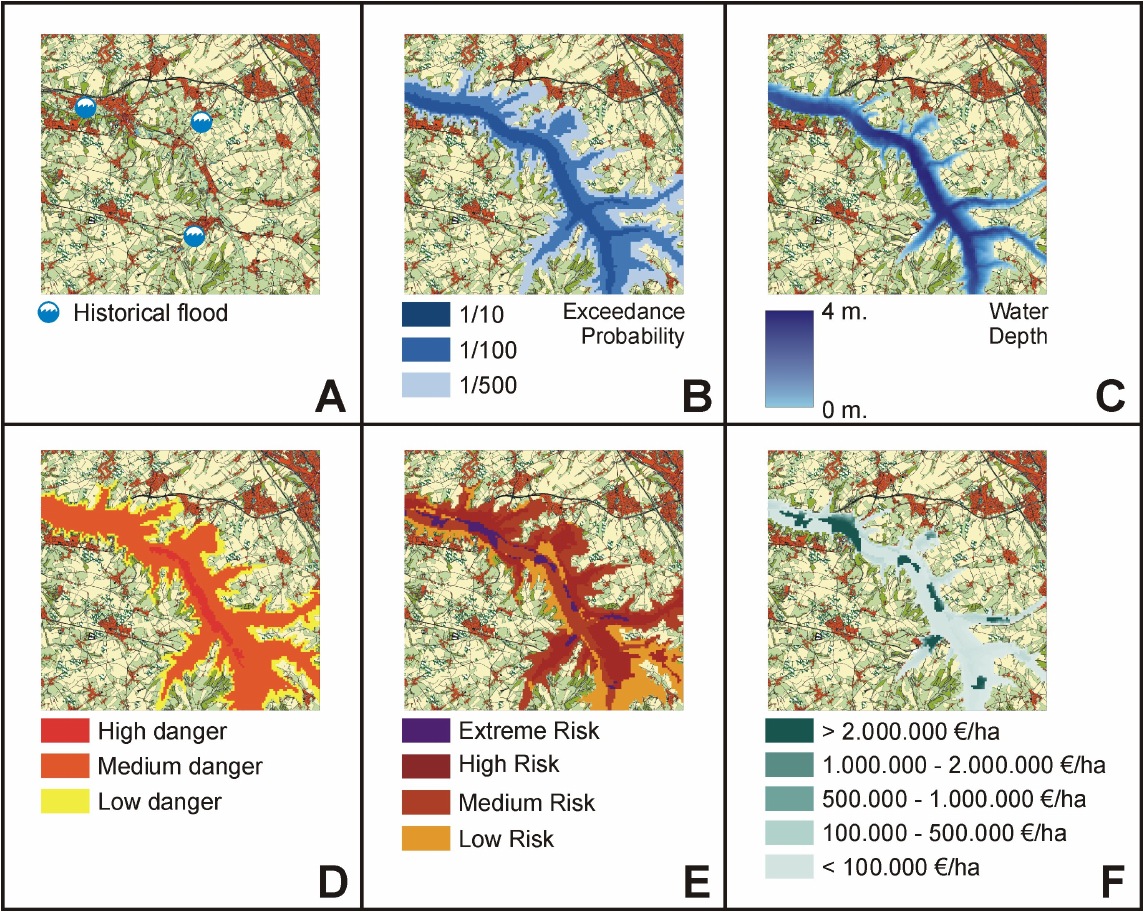
\includegraphics[width=\textwidth]{figures/flood_map_types}
    \decoRule
    \caption[Flood map types]{A depiction of 6 different flood map types, from  \citet{DeMoel2009}, Figure 2. Refer to \cref{sec:flood_map_types} for description of the panels.}
    \label{fig:flood_map_types}
\end{figure}



%------------------------------------
%	FUTURE EXTREME EVENTS
%------------------------------------
\section{Past, present and future of extreme climatological and hydrological events} \label{sec:future_extremes}

In the last century little to no change in average river runoff occurred for unmanaged rivers \citep{Dai2016, Dai2009}, and despite few studies indicating an increase in observed extreme streamflows and river flooding \citep{Mallakpour2015, Stevens2016}, these results can vary wildly from region to region \citep[see e.g.][]{Do2017}. Due to uncertainties in both the driving and the hydrological models \citep{Gosling2017, Donnelly2017}, there is no general agreement on the observed changes \citep{Kundzewicz2012, Hall2014, Robson2002, Kundzewicz2010}. In Europe, recent changes in flood timings in winter and spring have been highlighted by \citet{Bloschl2017a}, although the spatial variability of the signal is high, with \blockquote{earlier spring snowmelt floods in northeastern Europe, later winter floods around the North Sea and parts of the Mediterranean coast owing to delayed winter storms, and earlier winter floods in western Europe caused by earlier soil moisture maxima}.\\
Summing up the observed trends in flood hazard, the IPCC Fifth Assessment Report \citep[][section 3.2.7]{IPCCAR5WG2_3} states:
\blockquote{There is \textit{low confidence}, due to \textit{limited evidence}, that anthropogenic
climate change has affected the frequency and magnitude of floods
at global scale \citep{Kundzewicz2013}. The strength of the evidence
is limited mainly by lack of long-term records from unmanaged
catchments.}.

The Earth is currently undergoing a relatively rapid warming period which is, according to climate scientists, primarily linked to anthropogenic activity \citep{Anderegg2010, IPCC2013}. Climate change affects all aspects of the atmospheric system, including the events which are usually associated with floods, such as extremely strong or prolonged periods of rain. Increases in heavy precipitations are more correlated with the total amount of moisture in the air (growing by approximately 7\% \SI{}{\per \celsius} according to the Clausius-Clapeyron equation) than with changes in mean precipitation \citep{Allen2002}, so that increases in extreme rainfall might happen even in regions with decreasing total precipitation.\\
In the Fifth Assessment Report \citep[][section 12.4.5.5]{IPCC2013}, the IPCC Working Group 1 stated regarding extreme precipitation events:
\blockquote{Return Periods are projected to be reduced by
about 10 to 20\% \SI{}{\per\celsius} over the most of the mid-latitude land masses with larger reductions over wet tropical regions \citep{Kharin2013}. Hence, extreme precipitation events will very likely be more intense and more frequent in these regions in a warmer climate. Reductions in return values (or equivalently, increases in Return Period) are confined to convergent oceanic regions where circulation changes have reduced the available water vapour.}

This projected increase in extreme precipitation events all over the globe (see \cref{fig:ipcc_extreme_pr} for a map of changes) and in Europe in particular is supported by numerous studies \citep[e.g.][]{Christensen2004, Rajczak2013a, Pal2004, Durman2001, KleinTank2003, Fowler2003, Tramblay2018, Goubanova2007, Frei2006a, Pucik2017, Roudier2016, Gobiet2014} showing high likelihood of increasing frequency and/or intensity of such events before the end of the century, even in regions where the total precipitation is supposed to decrease.
\begin{figure}
    \centering
    \begin{subfigure}{.475\textwidth}
        \caption{}\label{fig:ipcc_extreme_pr/a}
        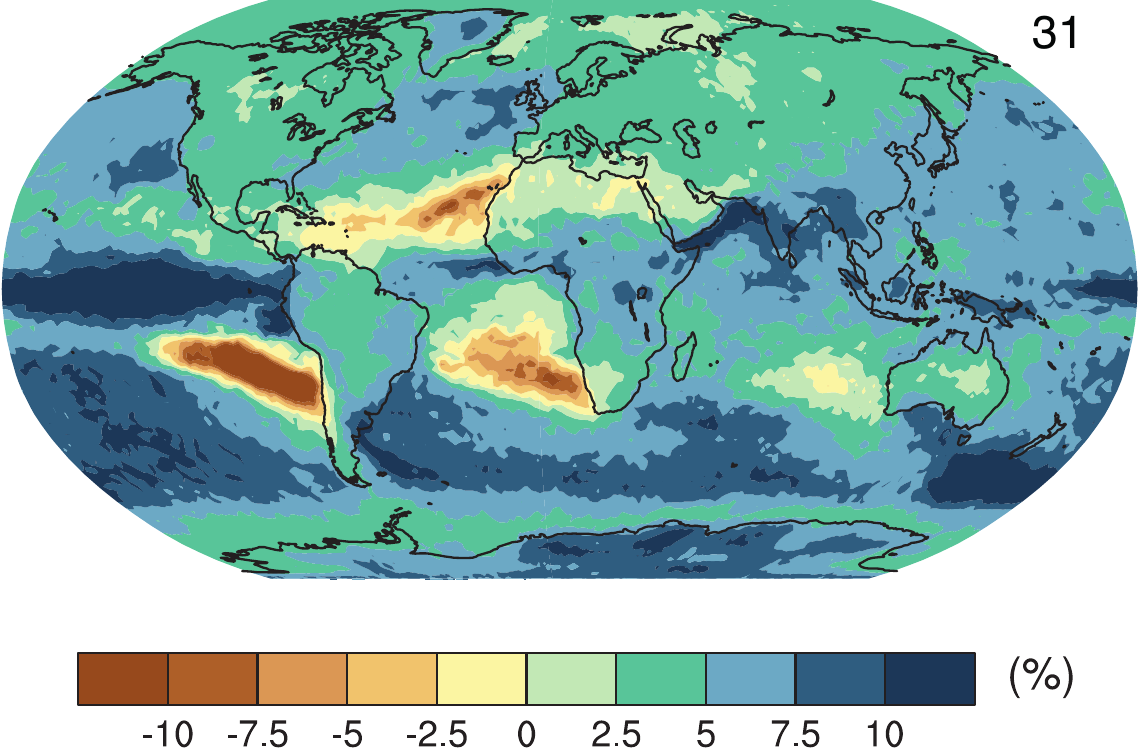
\includegraphics[width=\textwidth]{figures/extreme_pr_change/ipcc_extreme_pr_rp1.png}
    \end{subfigure}
    \begin{subfigure}{.475\textwidth}
        \caption{}\label{fig:ipcc_extreme_pr/b}
        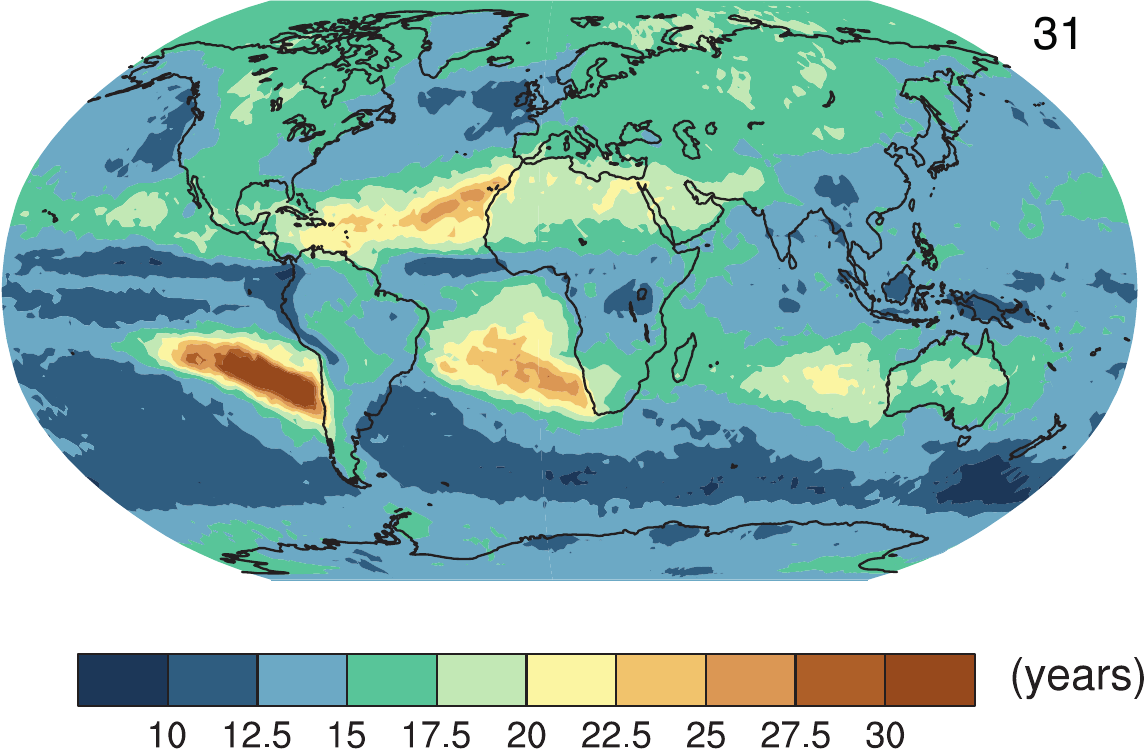
\includegraphics[width=\textwidth]{figures/extreme_pr_change/ipcc_extreme_pr_rp2.png}
    \end{subfigure}\\
    \decoRule
    \caption[Projected changes in extreme precipitation from IPCC AR5]{Annual maximum daily precipitation changes in an ensemble median of all CMIP5 models, according to \citet[section 12.4.5.5, figure 12.27]{IPCC2013}. \\
    In panel \subref{fig:ipcc_extreme_pr/a}, percent change in 20-year return values per \SI{1}{\celsius} of local warming, 2081--2100 relative to the 1986--2005 reference period.\\
    In panel \subref{fig:ipcc_extreme_pr/b}, the average 2081--2100 Return Period (in years) corresponding to the typical 1986--2005 20-year return values; regions of no change would have Return Periods of 20 years.
} \label{fig:ipcc_extreme_pr}
\end{figure}
As a consequence of the projected increment in extreme precipitation events, however, floods and flood-related damages are destined to rise in most areas of the world, despite improving flood protection infrastructures. The increase in risk is primarily due to higher exposure in flood-prone areas, which are on average very attractive for socioeconomic human activities (\cite{MunichRE2015, Kron2005, Hirabayashi2009, Mitchell2003, Barredo2009, Alfieri2016} and \cite[][section 3.4.8]{Aalst2014}).\\
\citet{Jongman2012} calculated that the total exposure to flood disasters, which is reported at \$\SIrange{27}{46}{\tera\nothing} globally in 2010, is going to more than triple (to \$\SIrange{80}{158}{\tera\nothing}) in 2050. In Europe, according to some studies ( \cite{Rojas2013, Alfieri2015, Forzieri2017} and \cite[][section 23.3.1.2]{IPCCAR5WG2_23}), the current annual population affected is expected to significantly increase by the 2080s, with annual damages growing up to 20-fold, if no change occurs in the current climate mitigation politics.
\citet{Forzieri2017} specifically estimates casualties related to river flood events to increase by 54\% (106 more lives claimed per year) under the A1B emission scenario \citep{IPCC2000SRES}. Multiple sectors are going to be affected, with worsening conditions in particular for electricity transport, road infrastructure and water and waste management \citep{Forzieri2018}.

As stated, the strongest driver for increasing flood risk is high exposure primarily due to growing population density. The other main factor, flood hazard, is also generally projected to increase according to the majority of studies, with the recently published IPCC Special Report ``Global Warming of  \SI{1.5}{\celsius}'' stating \citep[][section 3.3.5]{IPCC2018}: 
\blockquote{A global warming of 1.5°C would also lead to an expansion of the global land area with significant increases in runoff \textit{(medium confidence}) as well as to an increase in flood hazard in some regions (\textit{medium confidence}) compared to present day conditions.}

The projections are, however, very dependant on the region (or even basin) of interest, as local flood-related climatic characteristic can differ greatly from one location to another.
Global studies \citep{Hirabayashi2013, Arnell2016, Dankers2014, Hirabayashi2008, Alfieri2017, Milly2002}, for example, generally agree in finding increasing likelihood of flood events in the future for Southern Asia, Western Russia, Canada and the Northern Andes, but some highlight decreasing likelihood for most of Europe and the Amazon Basin (see e.g. \citet{Arnell2016, Hirabayashi2013, Dankers2014} and \cref{fig:future_flood}).
The resolution of such large scale studies, however, is usually not fine enough to resolve the details of some river catchments \citep{Whitfield2012, Gosling2011} especially for European basins, which are typically small in size.\\
Smaller scale studies over the European continent \citep[e.g.][]{Dankers2009, Alfieri2015a, Prudhomme2003, Alfieri2018, Feyen2012} generally find increasing flood hazard in most basins, especially in terms of higher frequency more than of higher magnitude \citep{Alfieri2015a, Lehner2006}, but large regional variations can be found due to different climatic characteristics.
As can be expected, the changes generally show strong seasonality, with increased discharges and frequency of flood events mostly concentrating in autumn and winter, and shifts in the flood regimes usually towards earlier and stronger winter floods \citep[e.g.][]{Middelkoop2001, Arheimer2015, coppola2014ChahydconPobasundglowar}.

\begin{figure}
    \centering
    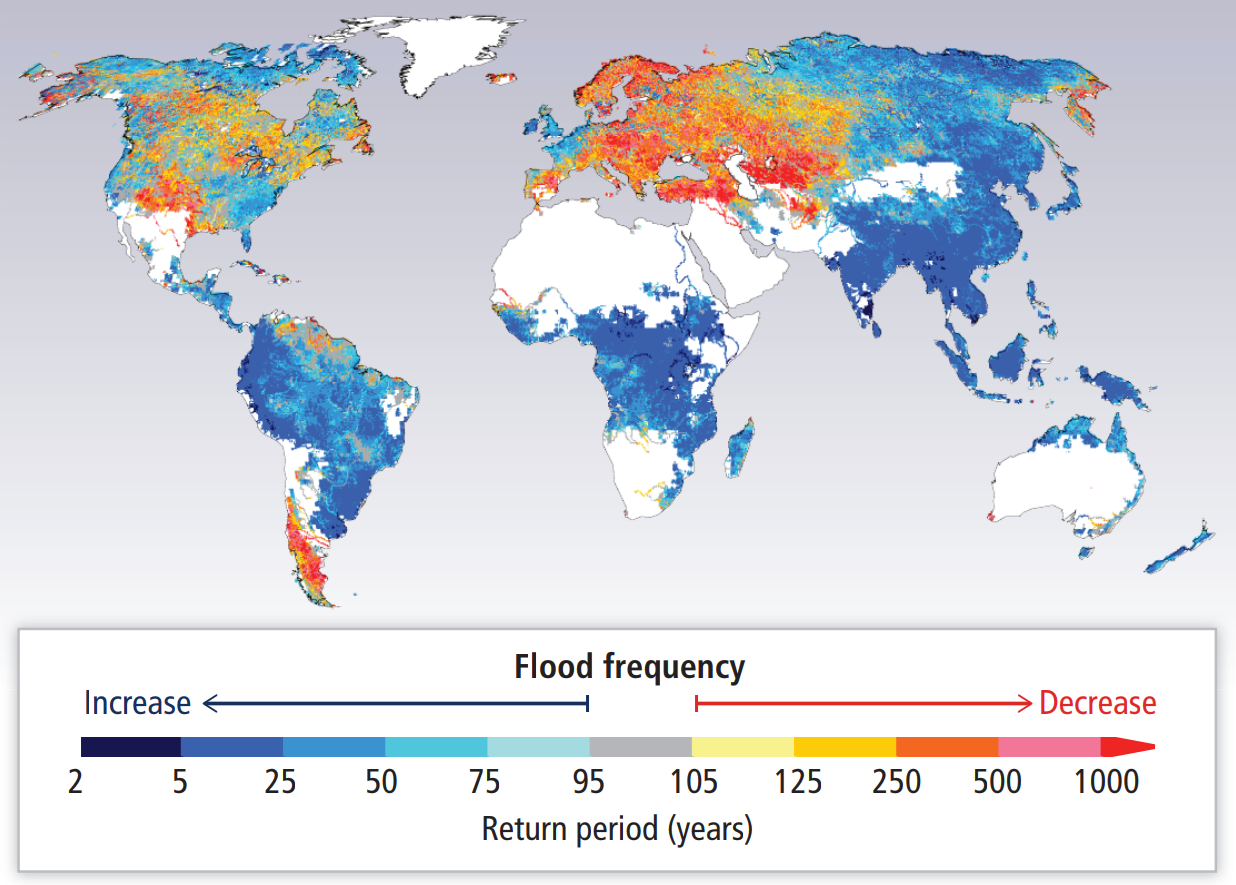
\includegraphics[width=\textwidth]{figures/Hirabayashi2013}
    \decoRule
    \caption[Future world flood hazard map]{Future world flood hazard map: 1971--2000 to 2071--2100 change as estimated by   \citet{Hirabayashi2013}, using 11 Coupled Model Intercomparison Project Phase 5 (CMIP5) models under the RCP8.5 (``business-as-usual'') scenario. Figure taken from \citet[][section 3.4.8]{Aalst2014}.}
    \label{fig:future_flood}
\end{figure}

\section{Flood hazard in the study domain}
This thesis focuses its attention specifically on flood hazard in Italy. The region is frequently affected by severe inundation events, with 584 reported casualties, 50 missing, 462 injured and 168254 evacuees in the last 50 years due to flooding only \citep[excluding flood-induced landslides, see][]{IRPI2018}. Observed heavy precipitation trends in the last century indicate a general decrease of total precipitation, but an increase in extreme events \citep{Brunetti2004, Brunetti2001, Brunetti2004a}. Recent flood events with several casualties, caused primarily by the inundation include floods in
Polesine (1951, 84 casualties),
Salerno (1954, 318),
Tuscany (1966, 34),
Piedmont (1994, 70),
Campania (1998, 159),
Piedmont (2000, 34),
Liguria (2011, 13),
Sardinia (2014, 18) and
Tuscany (2017, 9).\\
\Cref{fig:flood_events_ita}, obtained from the Polaris 2017 Periodic Report on Landslide and Flood Risk for the Italian Population \citep{IRPI2018}, shows the human costs (in terms of casualties and evacuees) in the period 1967--2016. The most affected regions is the  North-West, but catastrophic flood events occur all over Italy, having severely affected 920 out of 7982 municipalities in the last 50 years.

\begin{figure}
    \centering
    \includegraphics[width=0.9\textwidth]{figures/ita_flood/flood_ita_people_1967-2016}
    \decoRule
    \caption[Human costs of floods in Italy, 1967--2016]{Map of human costs for all flood events in Italy between 1967 and 2016. In dark blue are deaths, missing and injured; in light blue evacuees and homeless due to flooding events. Figure taken from \citet[][page 14]{IRPI2018}.}
    \label{fig:flood_events_ita}
\end{figure}

Despite the significant impact on the area, scientific studies concerning flood hazard estimation over the complete Italian domain are few: most works focus specifically on examining limited areas or basins \citep{Sole2008, Marchesini2016, Morelli2014, DiSalvo2017}, specific past events \citep{Marchi2010, Santo2012, Masoero2013, Amadio2013, Norbiato2007}, or target flood risk rather than hazard \citep{Salvati2010, Albano2017, Dottori2016}.

Some Italian regional protection agencies and basin authorities provide open-access flood hazard maps for their specific basin of interest. The Po River Basin Authority (AdbPo), for example, provides flood hazard maps for the whole Po basin (\cref{fig:flood_po}). These maps, however, have a few limitations for scientific work: they are rarely provided with accompanying vector data, the methodology is generally undisclosed, and maps from neighbouring agencies often do not agree with each other. Additionally, maps are often provided in numerous, separated image files with small extents, such as the maps provided by the Tevere River Basin Authority (ABTevere), which are comprised of 100 extremely small areas (\cref{fig:flood_tevere_union}). This fragmentation, while useful for small-scale studies, makes large-scale analysis much more difficult.

\begin{figure}
    \centering
    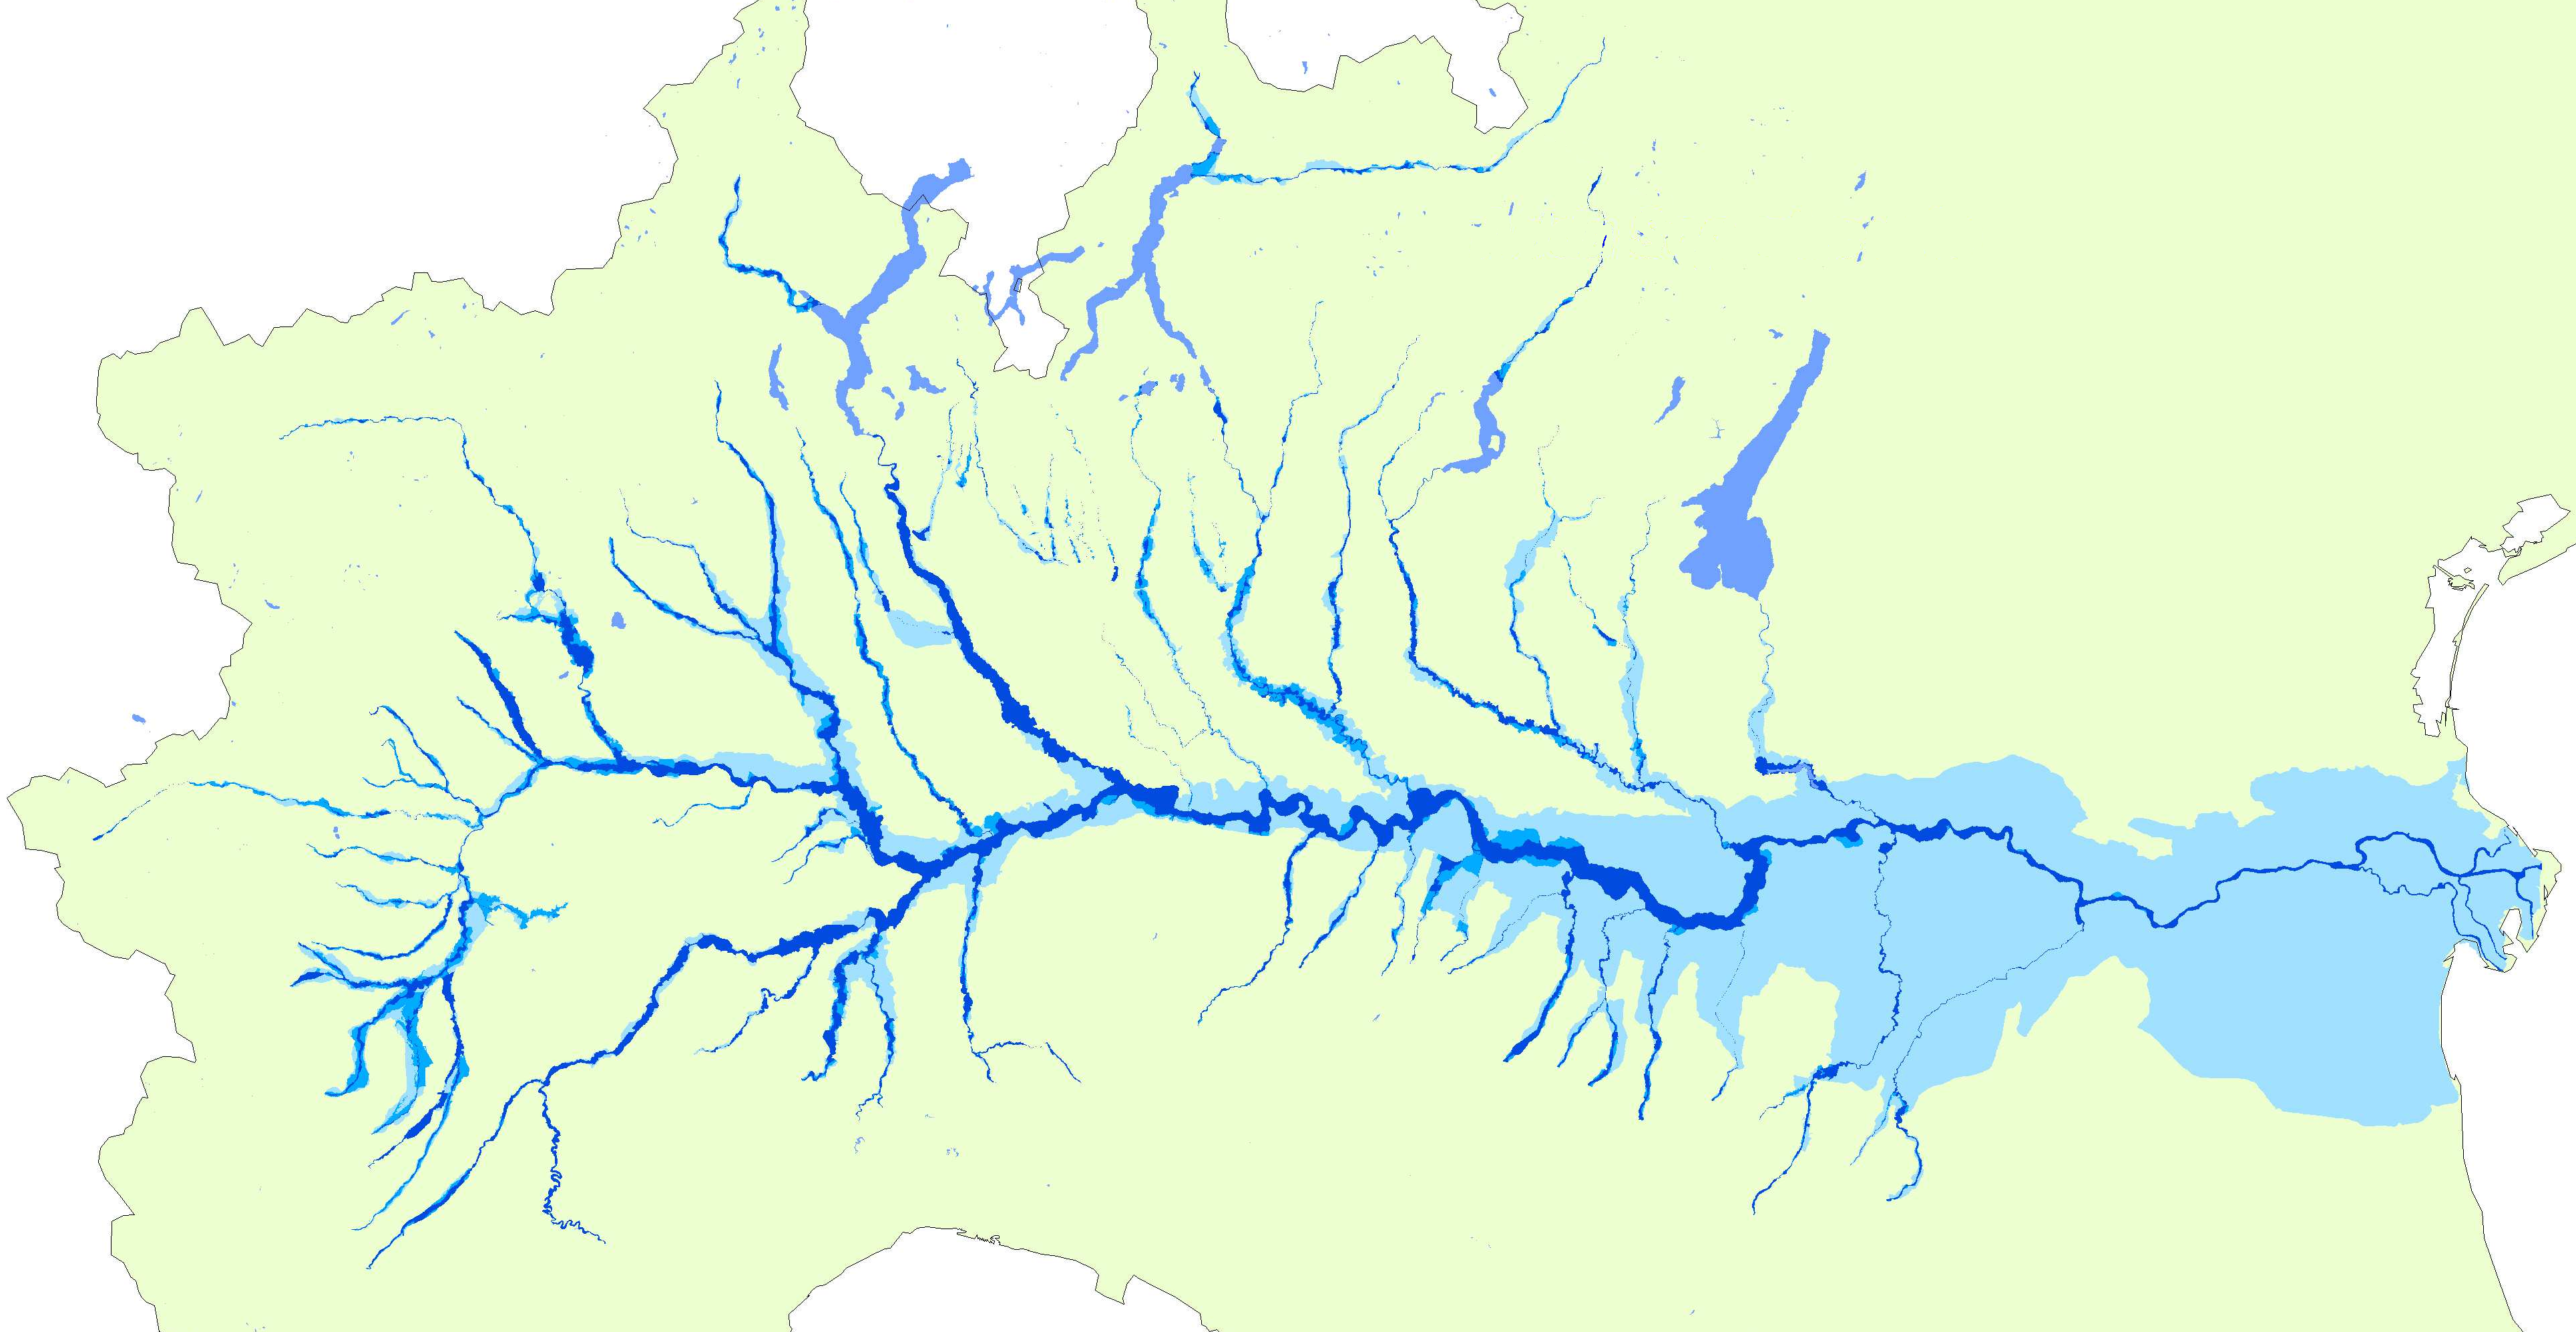
\includegraphics[width=\textwidth]{figures/ita_flood/po}
    \decoRule
    \caption[Flood hazard for the Po River Basin]{Flood hazard for the Po River Basin, as estimated by the Po River Basin Authority (AdbPo) (\url{http://www.adbpo.gov.it/}). Dark blue represents high flood hazard, with Return Period 10--20 years; medium blue 100--200 years; light blue 500 years. Open waters are in muted blue.}
    \label{fig:flood_po}
\end{figure}
\begin{figure}
    \centering
    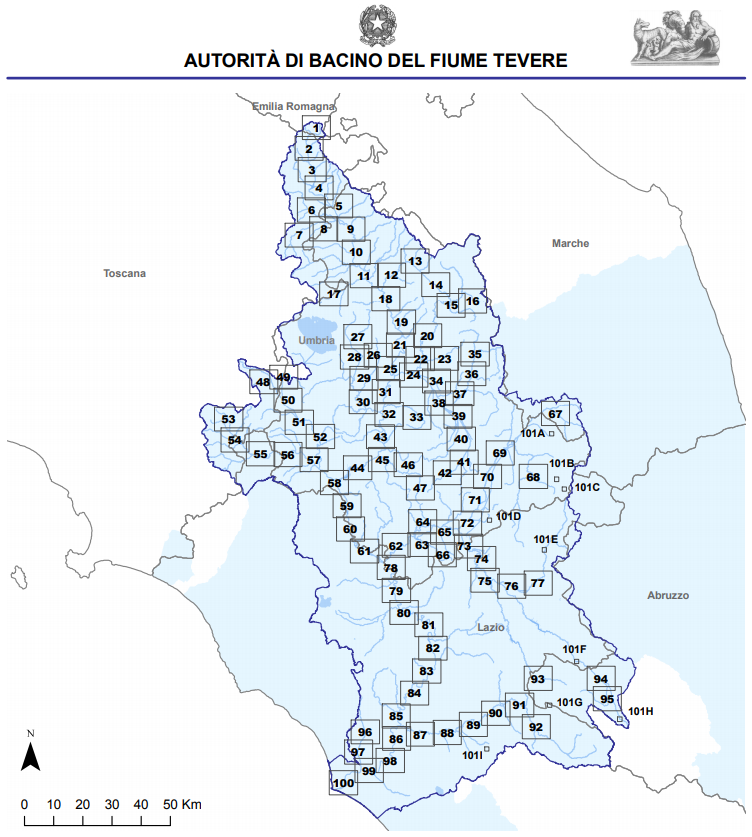
\includegraphics[width=0.5\textwidth]{figures/ita_flood/flood_tevere_union}
    \decoRule
    \caption[Union view of ABTevere flood map extents]{
    Union view of all 100 flood map extents provided by the Tevere River Basin Authority.
    From \url{http://www.abtevere.it}.
    }
    \label{fig:flood_tevere_union}
\end{figure}

A national, complete, and scientifically-based homogenised flood hazard map over Italy does not exist. The only nation-wide flood hazard product available is the report \textit{Dissesto idrogeologico in Italia: pericolosità e indicatori di rischio} \citep{ISPRA2018} from ISPRA, the Italian Superior Institute for the Ambient Protection and Research, in which the data from the single local agencies (often computed using undisclosed techniques) is merged and provided as vector data. Fluvial floods and storm surges are both considered, but no distinction is made in the output product.\\ \Cref{fig:ispra_ita_flood/a,fig:ispra_ita_flood/b,fig:ispra_ita_flood/c} show the ISPRA maps for high, medium and low hazard. The most affected areas are the Romagna, Valle D'Aosta, Piedmont, Lombardy and Tuscany regions, while the hazard is significantly lower towards the South and North-East of Italy. It is hard to discern whether regional differences (such as the increased risk in Valle D'Aosta compared to the neighbouring Piedmont or the relatively low hazard in the North-Eastern regions) come from real physical and meteorological diversities or from discrepancies in methodology and underlying data. \Cref{fig:ispra_ita_flood/d} shows the population count under a medium hazard category, grouped by municipality. Neighbourhoods of major cities, such as Turin, Milan, Venice and Rome, concentrate a large number of people in areas at risk of flooding, highlighting the importance, in these areas, of suitable emergency procedures and plans based on reliable data.
\begin{figure}
    \centering
    \begin{subfigure}{.475\textwidth}
        \caption{}\label{fig:ispra_ita_flood/a}
        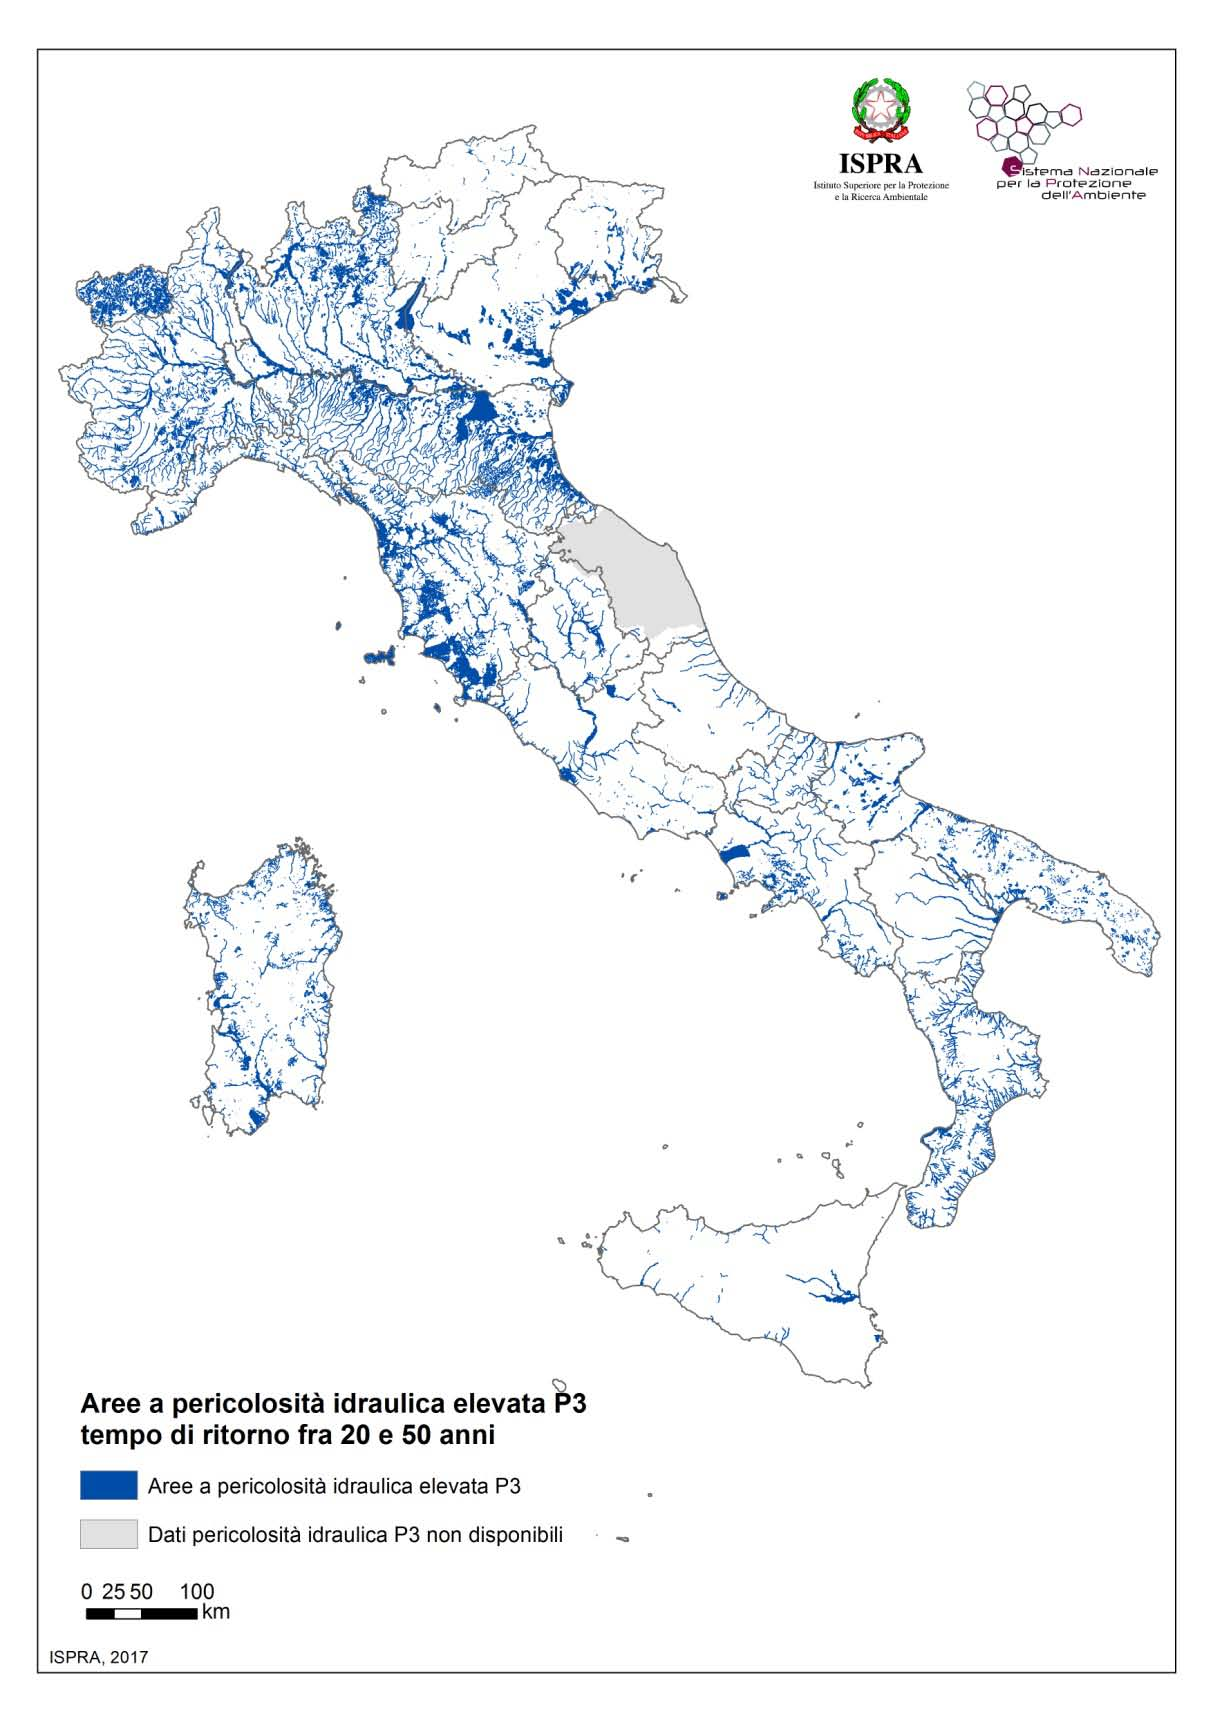
\includegraphics[width=\textwidth]{figures/ita_flood/p3}
    \end{subfigure}
    \begin{subfigure}{.475\textwidth}
        \caption{}\label{fig:ispra_ita_flood/b}
        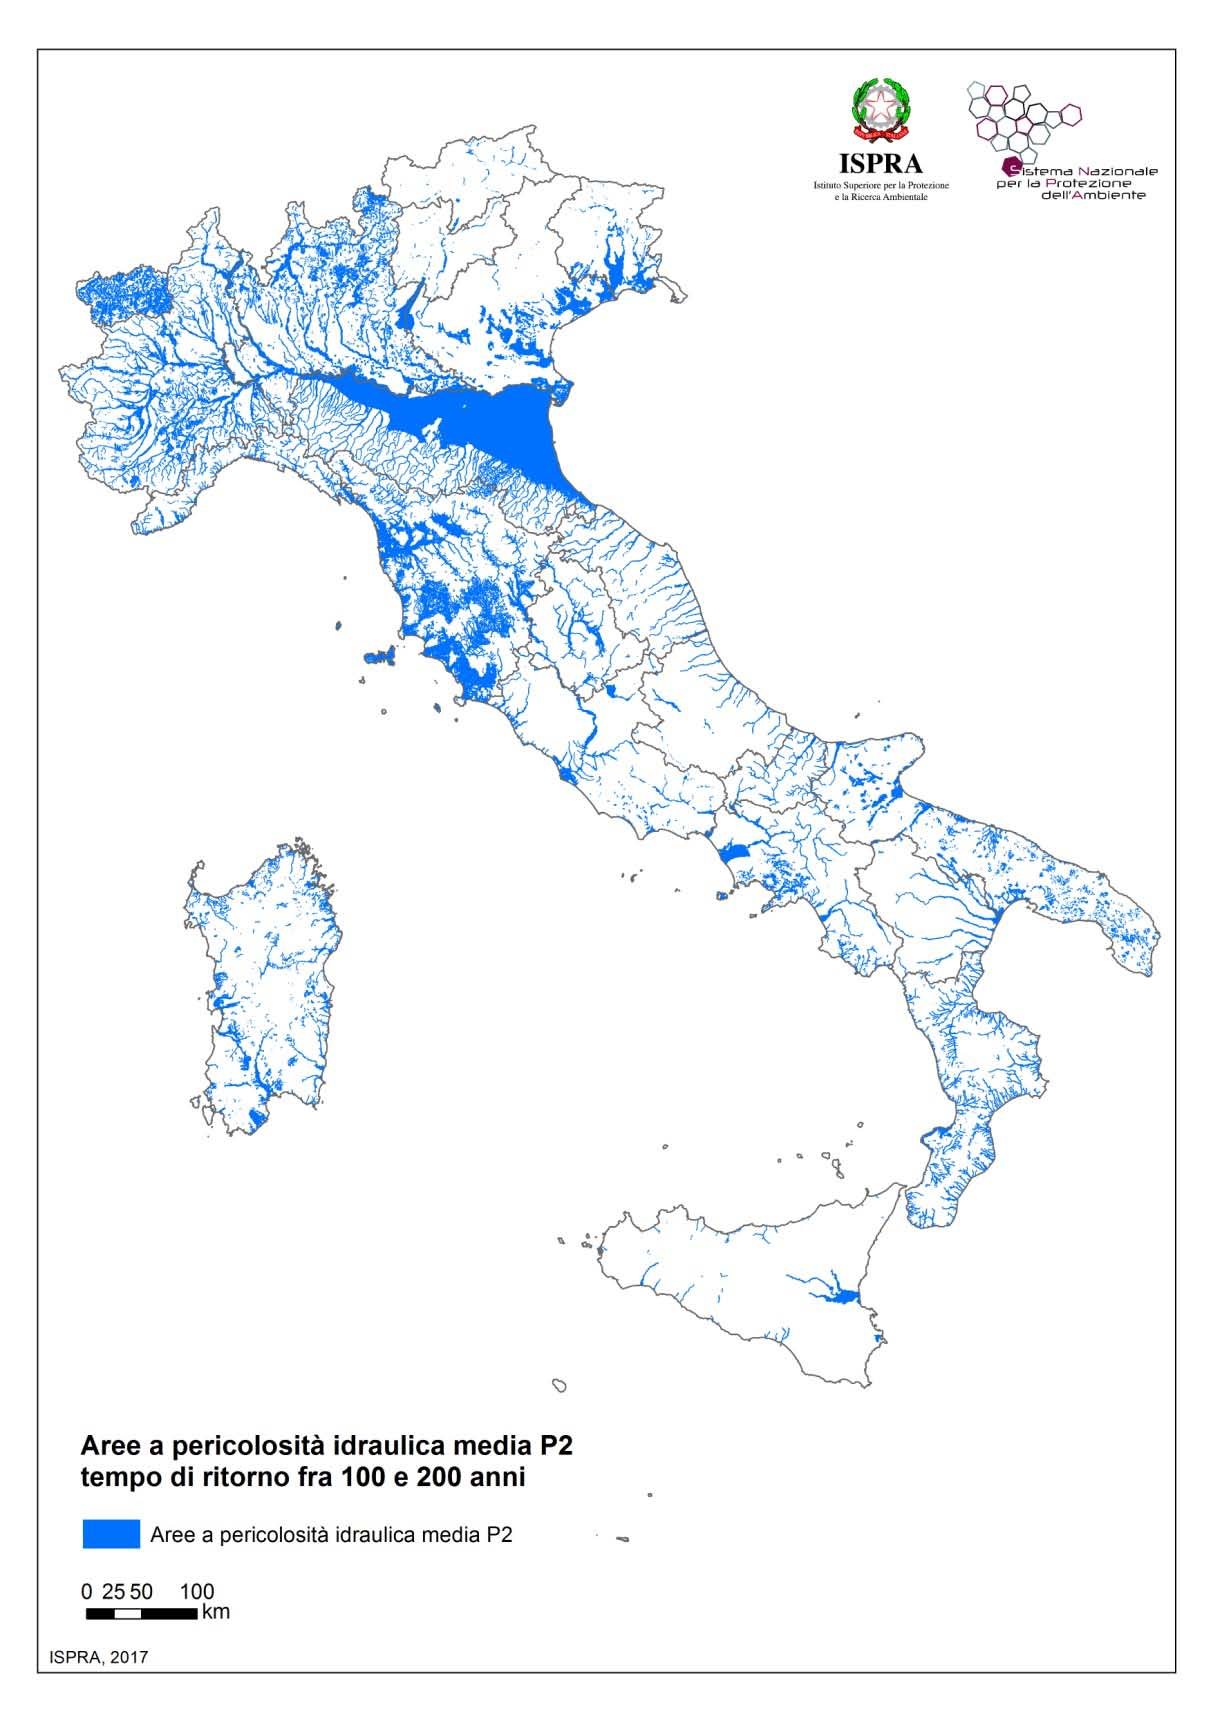
\includegraphics[width=\textwidth]{figures/ita_flood/p2}
    \end{subfigure}\\
    \begin{subfigure}{.475\textwidth}
        \caption{}\label{fig:ispra_ita_flood/c}
        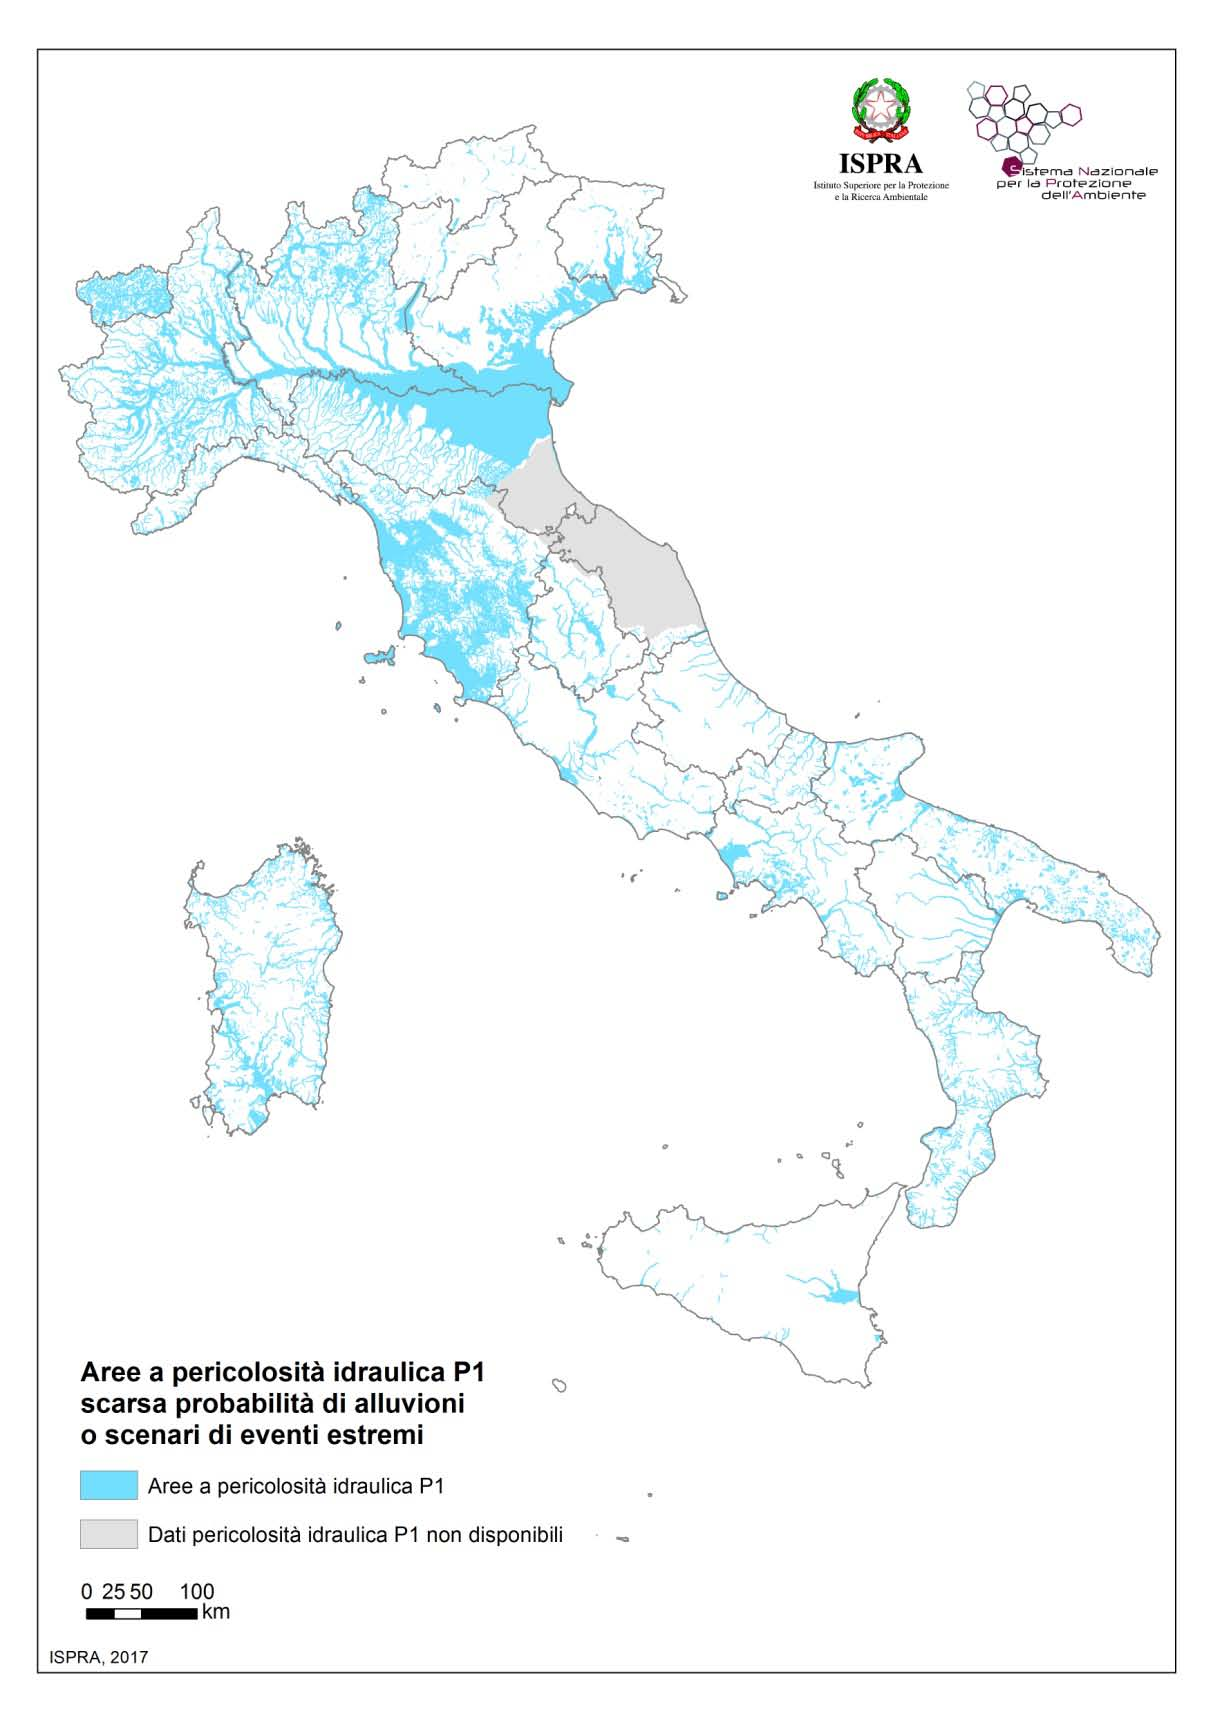
\includegraphics[width=\textwidth]{figures/ita_flood/p1}
    \end{subfigure}
    \begin{subfigure}{.475\textwidth}
        \caption{}\label{fig:ispra_ita_flood/d}
        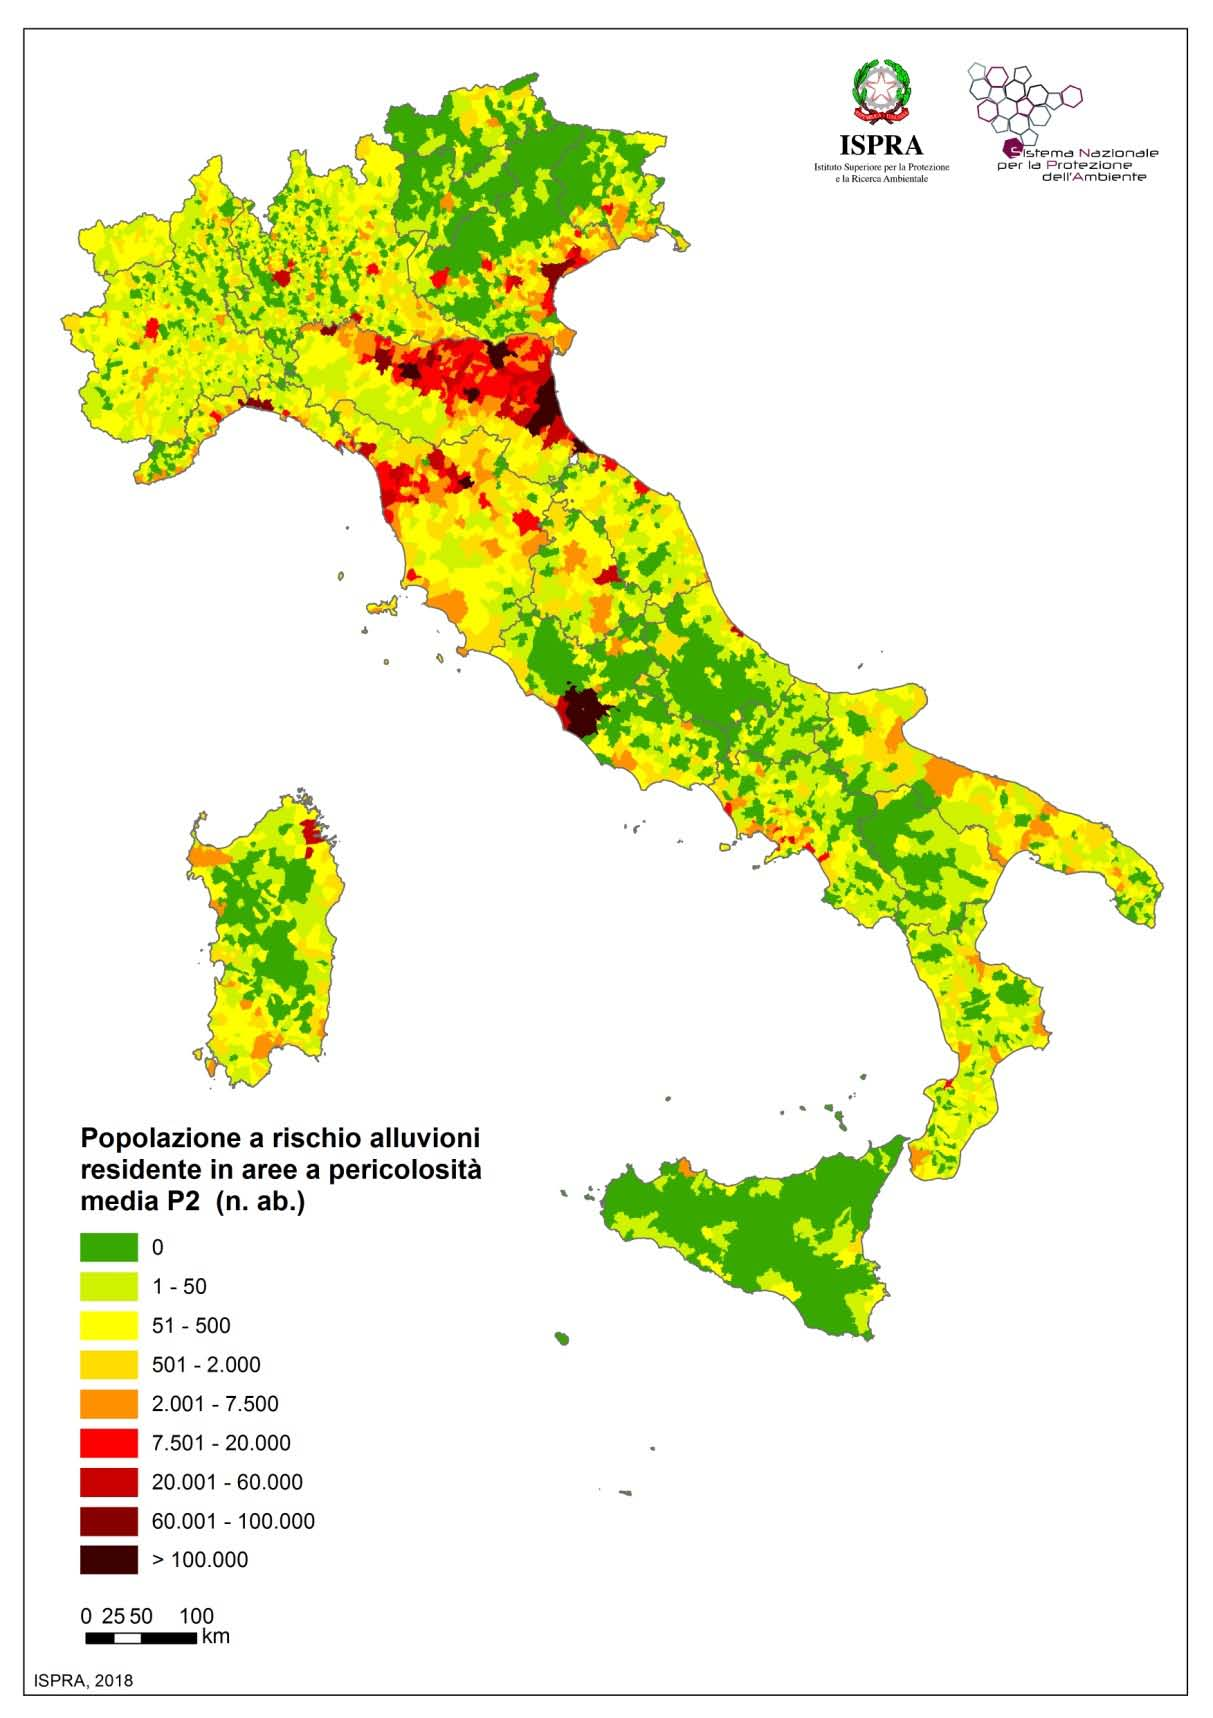
\includegraphics[width=\textwidth]{figures/ita_flood/pop_p2}
    \end{subfigure}
    \decoRule
    \caption[Flood hazard in Italy according to ISPRA]{
    Flood hazard in Italy, according to \citet[][figures 2.1 to 2.3 and 4.25]{ISPRA2018}. In panel \subref{fig:ispra_ita_flood/a}, areas with low flood Return Period (high hazard, 20--50 years); in panel \subref{fig:ispra_ita_flood/b}, medium Return Period (100--200 years); in panel \subref{fig:ispra_ita_flood/c}, high Return Period (``extremely rare events''). In panel \subref{fig:ispra_ita_flood/d}, the number of people exposed to a medium hazard, by municipality. Areas where data is missing are colored in grey.
} \label{fig:ispra_ita_flood}
\end{figure}
ISPRA estimates (\cref{tab:flood_risk_ita}) 10.4\% of the population, 12.4\% of the companies, 15.3\% of the cultural heritage and 8.4\% of the surface area of Italy to be currently at medium risk of inundation (Return Period of 100 to 200 years), with higher values in the North and significantly lower hazard in the South and Isles.

\newcolumntype{M}[1]{>{\centering\arraybackslash}m{#1}}
\begin{table}[]
\begin{tabular}{@{}rrM{1.25cm}M{1.25cm}M{1.25cm}M{1.25cm}M{1.25cm}M{1.25cm}@{}}
\toprule
                                ${\rm[ \% ]}$  & Hazard & N-W & N-E & Centre & South & Islands & Whole Italy \\ \midrule
\multirow{3}{*}{Population}        & High         & 2.9        & 7.1        & 3.6    & 2.2   & 1.2     & 3.5         \\
                                   & Medium       & 5.9        & 29.1       & 10.9   & 3.9   & 1.8     & 10.4        \\
                                   & Low          & 15.1       & 28.2       & 23.5   & 5.1   & 4.3     & 15.7        \\ \\
\multirow{3}{*}{Families}          & High         & 3.0        & 7.1        & 3.5    & 2.2   & 1.2     & 3.6         \\
                                   & Medium       & 6.1        & 29.6       & 10.9   & 3.8   & 1.9     & 10.8        \\
                                   & Low          & 15.3       & 28.7       & 23.7   & 5.0   & 4.4     & 16.3        \\ \\
\multirow{3}{*}{Buildings}         & High         & 2.9        & 6.6        & 3.8    & 2.4   & 1.3     & 3.4         \\
                                   & Medium       & 5.9        & 25.8       & 10.7   & 3.4   & 2.0     & 9.3         \\
                                   & Low          & 16.0       & 25.7       & 22.1   & 4.6   & 4.2     & 14.1        \\ \\
\multirow{3}{*}{Companies}         & High         & 3.8        & 7.3        & 4.0    & 2.2   & 1.6     & 4.1         \\
                                   & Medium       & 7.1        & 29.9       & 13.2   & 4.4   & 2.4     & 12.4        \\
                                   & Low          & 16.3       & 27.7       & 28.5   & 5.8   & 5.2     & 18.4        \\ \\
\multirow{3}{*}{\parbox{2cm}{\raggedleft Cultural heritage}} & High         & 9.8        & 11.9       & 3.2    & 2.5   & 2.4     & 6.8         \\
                                   & Medium       & 14.2       & 33.7       & 8.4    & 3.3   & 3.0     & 15.3        \\
                                   & Low          & 23.7       & 34.4       & 14.0   & 4.0   & 4.8     & 19.4    \\
\bottomrule
\end{tabular}
\caption[Percentages of categories at risk of flooding]{Estimated percentage of population, families, buildings, companies and cultural heritage at three flood hazard levels, divided by Italian macroregion. High hazard corresponds to an estimated Return Period of 20--50 years; medium to 100--200 years; low to ``extremely rare events''. Macroregions are defined as follows:\\
N-W: Piedmont, Valle D'Aosta, Lombardy and Liguria; N-E: Trentino--Alto Adige, Veneto, Friuli--Venezia Giulia, Emilia--Romagna; Centre: Tuscany, Umbria, Marche, Lazio; South: Abruzzo, Molise, Campania, Puglia, Basilicata, Campania; Islands: Sicily, Sardinia.\\
Data from \citet{ISPRA2018}.}\label{tab:flood_risk_ita}
\end{table}

Although no official national study on the topic is available, in the future flood hazard is generally projected to increase in the region by several European-wide studies, in contrast with the results of some global studies (see \cref{fig:future_flood}), albeit strong differences exist among the available studies. Most works focus on estimating the change in flood hazard by focusing on the intensity or recurrence time of extreme discharges, most often $Q_{100}$, the typical 100 year Return Period discharge.\\
\Citet{Rojas2012} uses an ensemble of 12 bias-corrected simulations from the ENSEMBLES project to drive a single calibrated hydrological model (LISFLOOD) over all of Europe. Due to the large spatial extent, the study resolution is relatively low (\SI{5}{\kilo \metre}), thus reproducing only major rivers, which are not necessarily those contributing the most to flood hazard.
The results (\cref{fig:rojas_change}) generally indicate an increase in 100 year Return Period peak discharges (and thus flood intensity) under a climate change scenario (SRES A1B), when comparing the future (2071--2100) to the control period (1961--1990).
The change is, however, strongly dependent on the model and the region of interest.
In Italy, the rivers showing the greatest increase (and agreement between the 12 simulations) are those located in the North and fed by the Alpine range; changes in the Centre and South (both positive and negative) show lower agreement between models.\\
In a similar study, \citet{Thober2018} employs a multi-model ensemble of three hydrological models forced by five Global Climate Models under three different warming levels (1.5, 2 and \SI{3}{\celsius}). The climate change results are generally in agreement with \citep{Rojas2012} (despite some differences, especially in Scandinavia and the Baltic Republics), finding reduced flood hazard for Eastern Europe and Mediterranean regions, but increased hazard for North Italy (\cref{fig:thober_change}).\\
\citet{Feyen2012, Dankers2009} show more conflicting results for Italy, with only the Po river seemingly subject to increased extreme peak discharges. In some studies \citep{Roudier2016, Donnelly2017, Alfieri2015, Alfieri2015a}, on the other hand, a more uniform increase in high runoff events all over Western and Southern Europe and the Mediterranean is found (see e.g.\ figures \ref{fig:donnelly_change} and \ref{fig:alfieri_change}). In these studies, the whole Italian territory shows a marked increase in flood-related variables, although the change in the Northern basins remains more evident.

The spatial (usually \SI{5}{\kilo\meter}) and temporal (daily) resolution of the cited works is generally too low to capture the details of smaller river basins: the maps reported in these studies in fact only show major rivers in Italy. In this thesis work, which focuses only on the Italian domain, higher resolutions are possible while keeping the computational costs reasonable.

\begin{figure}
    \centering
    \begin{subfigure}{\textwidth}
        \caption{}\label{fig:rojas_change/a}
        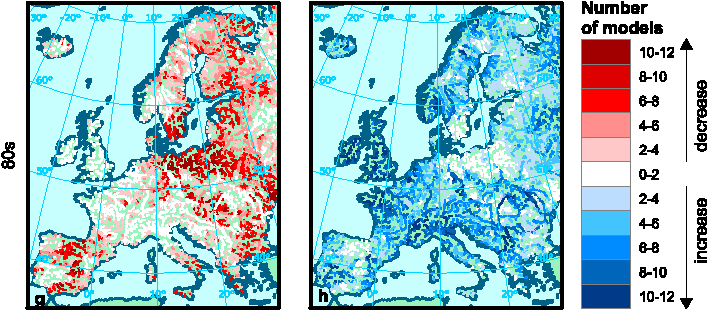
\includegraphics[width=\textwidth]{figures/ita_flood/rojas2_crop}
    \end{subfigure}\\
    \begin{subfigure}{\textwidth}
        \caption{}\label{fig:rojas_change/b}
        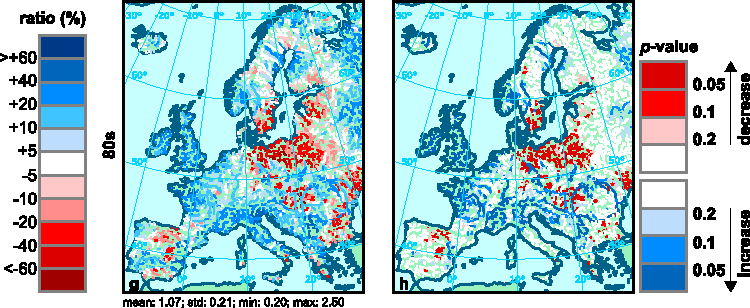
\includegraphics[width=\textwidth]{figures/ita_flood/rojas3_crop}
    \end{subfigure}
    \decoRule
    \caption[Extreme discharge change in Europe according to \citet{Rojas2012}]{
    Change in extreme discharge ($Q_{100}$: peak annual discharge with 100 year Return Period), extracted from \citet[][figures 5 and 6]{Rojas2012}. In the upper panels, the number of models agreeing in a decrease (left) or increase (right) in $Q_{100}$ discharges by the end of the century, compared to the control period. In the lower panels, ensemble average of the change (left) and p-value of the signal (right).
} \label{fig:rojas_change}
\end{figure}

\begin{figure}
    \centering
    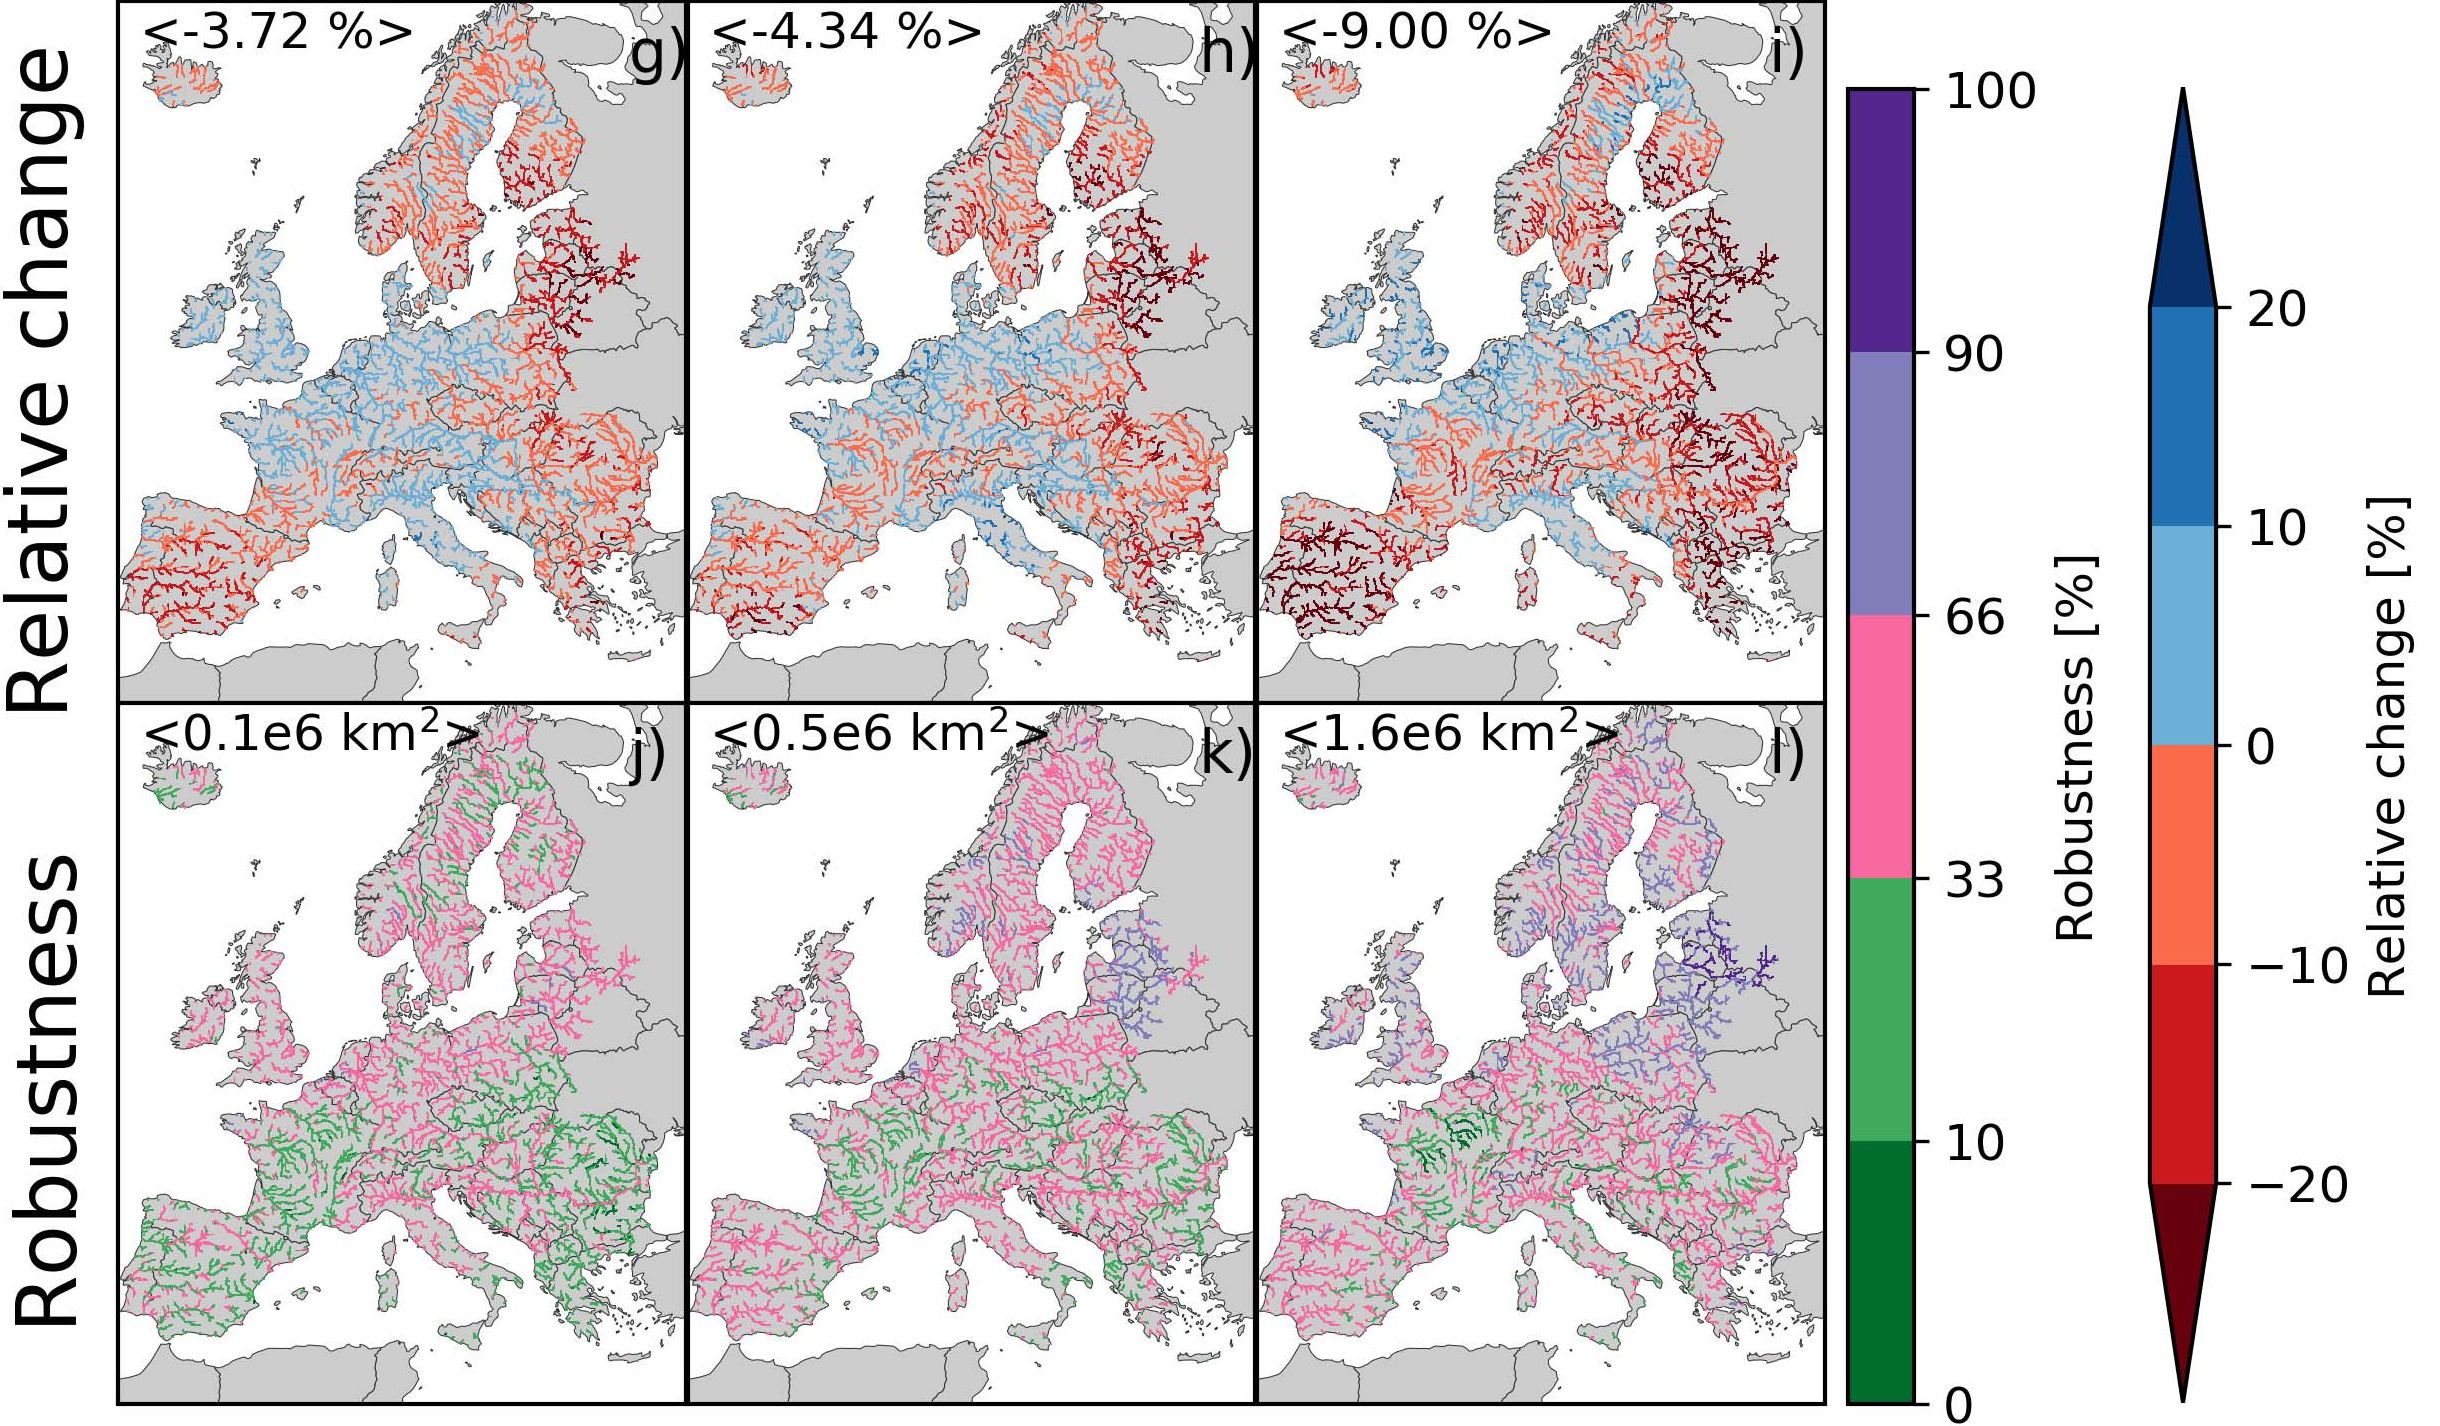
\includegraphics[width=\textwidth]{figures/ita_flood/thober}
    \decoRule
    \caption[High runoff change in Europe according to \citet{Thober2018}]{
        Change in high runoff (mean annual maximum runoff), extracted from \citet[][figure  1]{Thober2018}. The three columns represent the three warming targets considered: +\SI{1.5}{\celsius}, +\SI{2}{\celsius} and  +\SI{3}{\celsius}. In the top panel, the relative change compared to the reference period (1971--2000) and, in brackets, the spatial average. In the bottom panel, the percentage of ensemble members indicating robust changes and, in brackets, the area exhibiting changes with likelyhood greater than 66\%.
    }
    \label{fig:thober_change}
\end{figure}

\begin{figure}
    \centering
    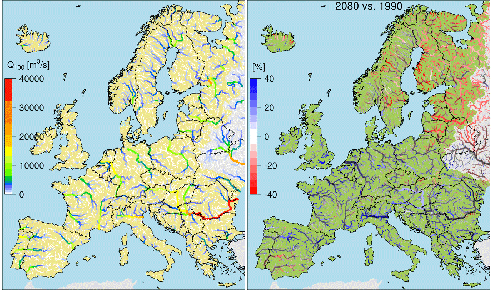
\includegraphics[width=\textwidth]{figures/ita_flood/alfieri2015_crop}
    \decoRule
    \caption[Extreme discharge change in Europe according to \citet{Alfieri2015a}]{
        Extreme discharge ($Q_{100}$: peak annual discharge with 100 year Return Period), extracted from \citet[][figure  6]{Alfieri2015a}. In the left panel, ensemble mean of the reference period (1976--2005); in the right panel, percentage change for the time slice  2066--2095.
    }
    \label{fig:alfieri_change}
\end{figure}

\begin{figure}
    \centering
    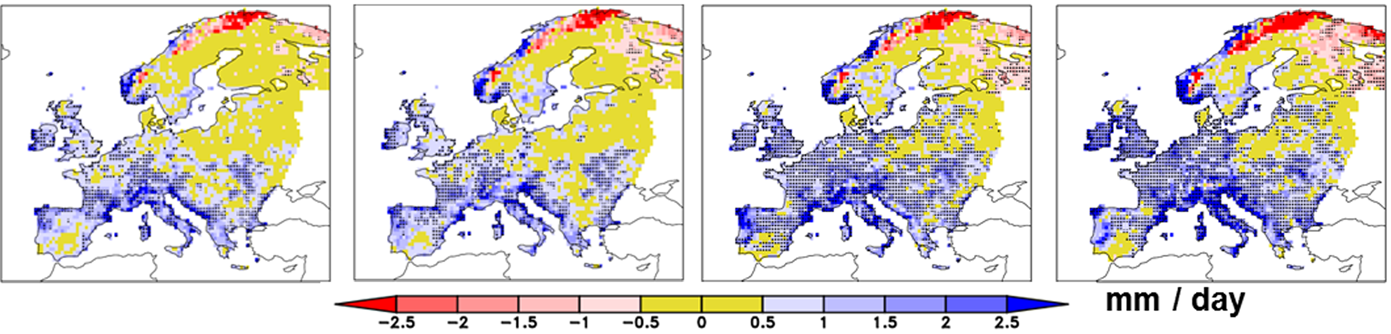
\includegraphics[width=\textwidth]{figures/ita_flood/donnelly}
    \decoRule
    \caption[High runoff change in Europe according to \citet{Donnelly2017}]{
        Change in high runoff (mean annual maximum runoff), extracted from \citet[][figure  4]{Donnelly2017}. The four columns represent the four warming scenarios considered: +\SI{1.5}{\celsius} with RCP 2.6 and 4.5, +\SI{2}{\celsius} with RCP 2.6 and 4.5, +\SI{2}{\celsius} with RCP 4.5 and 8.5, +\SI{3}{\celsius} with RCP 4.5 and 8.5.
    }
    \label{fig:donnelly_change}
\end{figure}


%------------------------------------
%	TODO STUFF
%------------------------------------
% \section{Additional sources to integrate in this chapter}
% \begin{itemize}
% \item check all TODOs
% \item read again \url{http://ec.europa.eu/environment/water/flood_risk/flood_atlas/pdf/handbook_goodpractice.pdf}
% \item include citation EU Floods Directive (2007/60/EC) , \cite{Mysiak2013, EUFD2007}
% \item section to talk about uncertainties? \citet{alfieri2014} has a good section about it
% \item Alps are the water tower of the Po plain, and for this reason I might want to give them a closer look. I could cite one of the many kotlarski works, or e.g. \citet[][]{Gobiet2014}. View the 'Alps' category in my Mendeley, it contains about 30 works on the subject
% \end{itemize}